\section{Estimating road speeds}
\label{sec:vehicle_speeds}

Now that we have estimated the necessary vehicle states and their respective trajectories, we can infer each vehicle's \emph{average speed} along road segment $\ell$ of its current route, $\Vtt_{\ell}$. These estimates are later used to update the \emph{road network state} (\cref{cha:network_model}) and ultimately estimate arrival times (\cref{cha:prediction}).


Estimation of average road speed is performed by first computing the \emph{travel time} along each road segment as the bus traverses the network. To do so, we record the time when the vehicle starts and ends each segment, $\Vsegstart_\ell$ and $\Vsegend_\ell$, respectively, and take the difference to obtain the travel time in seconds. By using a particle filter, we record these values for each particle as it is transitioned to each new state. Finally, transforming to average speed uses the length of the segment, $\Tseglen_\ell$, in meters, and the standard speed formula ($\text{speed} = \frac{\text{distance}}{\text{time}}$):
\begin{equation}
\label{eq:vehicle_avg_speed}
\Vtt\vi_\ell = \frac{\Tseglen_\ell}{\Vsegend\vi_\ell - \Vsegstart\vi_\ell}.
\end{equation}


Since estimating \cref{eq:vehicle_avg_speed} is straightforward for each particle, the posterior distribution of the vehicle's average travel time along segment $\ell$, given all observations up to and including time $\Vtime_k$, is approximated using the Dirac delta measure,
\begin{equation}
\label{eq:pf_speed_dist}
p(\Vtt_\ell | \Vobs_{1:k}) \approx
\sum_{i=1}^\Np \Pwt_k \DiracMeasure{\Vtt\vi_\ell}{\Vtt_\ell}.
\end{equation}
In situations where only some particles have completed travel along a segment, the application waits until the next iteration to re-check that all particles have completed it and, if so, the average speed is calculated.


\subsection{Simulation study}
\label{eq:pf_simulation_study}

To assess the accuracy of the models presented in \cref{sec:vehicle_model}, vehicle simulations were performed with known road speeds while tracking the vehicle along the route. Three different sampling methods were used to obtain observations:
\begin{itemize}
\item uniform sampling with 10~second intervals;
\item uniform sampling with 30~second intervals; and
\item non-uniform sampling at nodes.
\end{itemize}
As mentioned in \cref{sec:vp_data}, the last of these is, in fact, a common feature of the Auckland Transport data; we discuss the complications further in \cref{sec:pf_implementation}. In each simulation, we implemented the three variations of the transition function: $\Vtrans_{A1}$, $\Vtrans_{A2}$, and $\Vtrans_{A3}$.


The posterior mean travel time was used to examine and compare the estimation accuracy of the models, which is simple to calculate from the particle filter estimates of travel time using the weighted mean of the sample (\cref{app:particle-summaries}):
\begin{equation}
\label{eq:pf_travel_time_mean}
\bar\Vtt_\ell =
\E{\Vtt_\ell | \Vobs_{1:k}} =
\sum_{i=1}^\Np \Pwt_k \Vtt\vi_\ell.
\end{equation}


To evaluate and compare the estimation performance of the models, we use \gls{rmse} and \gls{mae} (defined in \cref{app:error-functions}).


\subsubsection{Simulation A: general vehicle model}
\label{sec:vehicle_sim_A}





The simulated data, shown in \cref{fig:sim1_graph}, uses the transition model described by $\Vtrans_{A3}$ to simulate a vehicle trajectory ignoring bus stops. Observations are obtained using three sampling methods: uniform sampling with high and low frequency, and non-uniform sampling, which is more in line with how the Auckland Transport data is collected.


The goal of the simulation is to estimate the vehicle's average speed along several road segments, as well as the associated uncertainty. The simulation was performed in \Rstats{} \citep{rcore} using $\Np = 2000$ particles per vehicle, and so the implementation is slightly different from the \Cpp{} one defined in \cref{sec:pf_implementation}.

\begin{knitrout}\small
\definecolor{shadecolor}{rgb}{0.969, 0.969, 0.969}\color{fgcolor}\begin{figure}
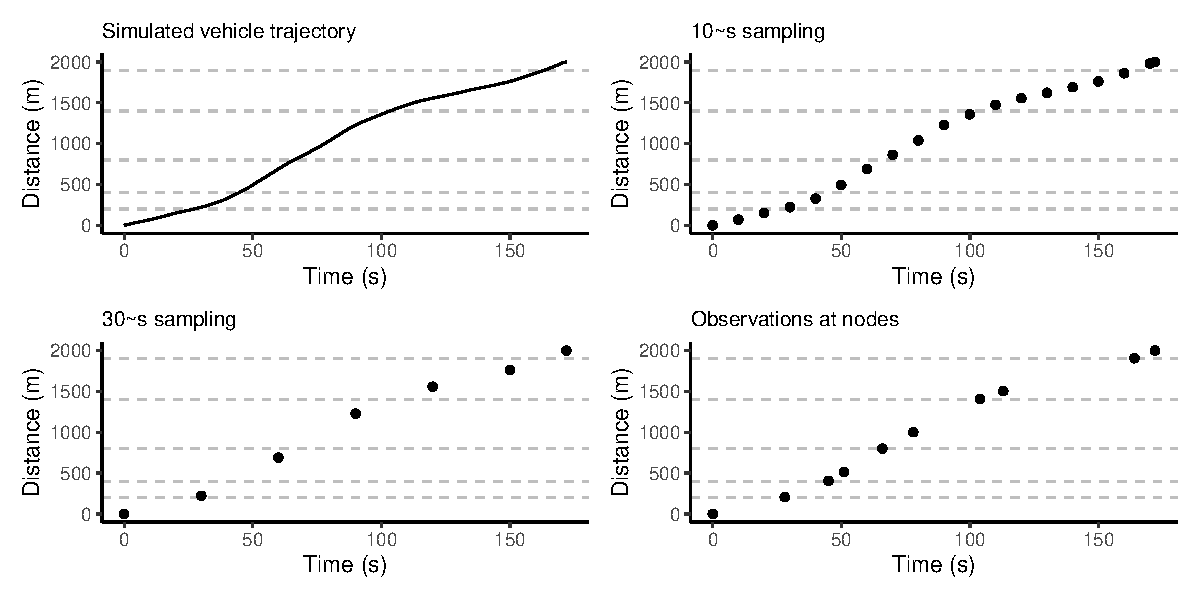
\includegraphics[width=\linewidth]{figure/sim1_graph-1} \caption[Simulated vehicle trajectory, with five full road segments, along with simulated observations with three sampling techniques]{Simulated vehicle trajectory, with five full road segments, along with simulated observations with three sampling techniques.}\label{fig:sim1_graph}
\end{figure}


\end{knitrout}

\begin{knitrout}\small
\definecolor{shadecolor}{rgb}{0.969, 0.969, 0.969}\color{fgcolor}\begin{figure}
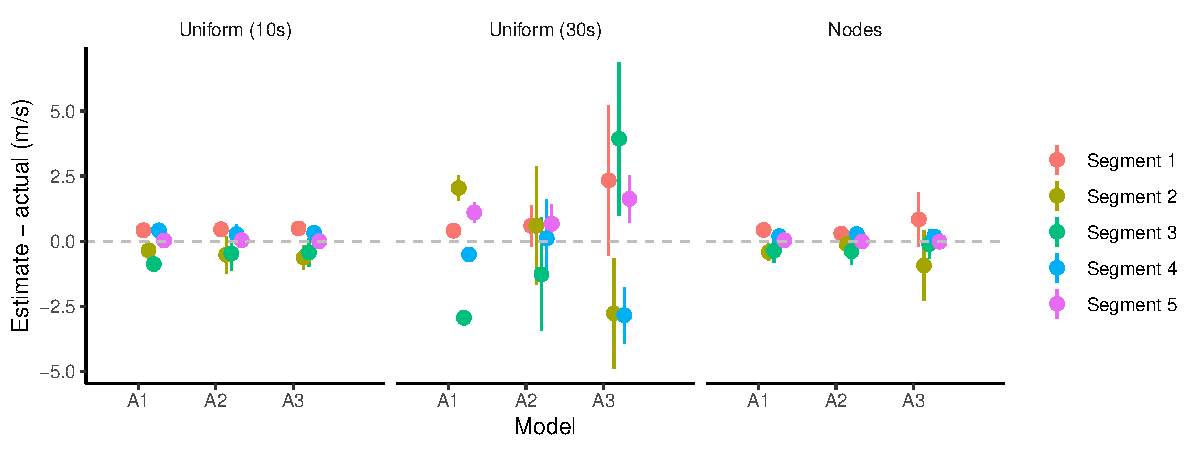
\includegraphics[width=\linewidth]{figure/sim1_pf-1} \caption[Simulation results for the three models (rows) applied to the data from three sampling methods (columns), using $\Np=2000$ particles]{Simulation results for the three models (rows) applied to the data from three sampling methods (columns), using $\Np=2000$ particles. The standard deviation of the particle travel times is represented as error bars, though in many cases the error is too small to display.}\label{fig:sim1_pf}
\end{figure}


\end{knitrout}


The results of the simulation applied to the data displayed in \cref{fig:sim1_graph} is shown in \cref{fig:sim1_pf}. Under the high-frequency uniform sampling method, all models perform similarly with high precision (the errors are all close to zero) and accuracy (the uncertainty is small enough that the error bars are barely visible). For the low-frequency sampling, however, model A2 shows slightly better precision than A1 and A3. Finally, for sampling at nodes, the models all perform similarly.



To further examine the comparative performance of the models, we repeated the simulation 100~times using the same segments and sampling points, but varying the underlying trajectory of the vehicle, with the results displayed in \cref{fig:sim1_pf_full}. Models A1 and A2 have better accuracy than A3. Most obviously, however, is that the sampling rate significantly affects accuracy. An overall comparison of \gls{rmse} and \gls{mae} are displayed in \cref{tab:sim1_pf_full}, which affirms the findings that A3 is less accurate than the other methods  (except under high-frequency sampling where they all perform similarly).


\begin{knitrout}\small
\definecolor{shadecolor}{rgb}{0.969, 0.969, 0.969}\color{fgcolor}\begin{figure}
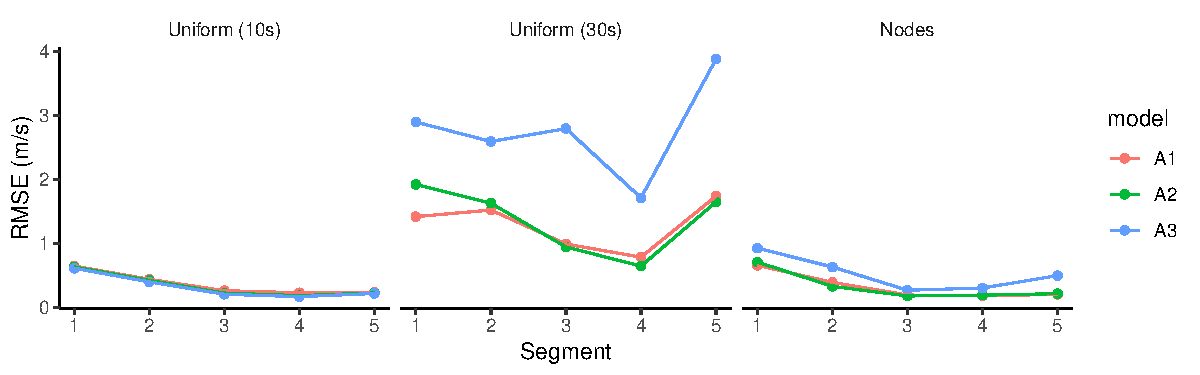
\includegraphics[width=\linewidth]{figure/sim1_pf_full-1} \caption[Speed estimation results for 100 simulations]{Speed estimation results for 100 simulations. In each the vehicle trajectory is simulated using a different seed, and the speed estimate is taken as the mean of the particle speeds along each segment.}\label{fig:sim1_pf_full}
\end{figure}

\begin{table}

\caption{\label{tab:sim1_pf_full}RMSE of average speed estimation}
\centering
\fontsize{8}{10}\selectfont
\begin{tabular}[t]{llrr}
\toprule
Sampling method & Model & RMSE (m/s) & MAE (m/s)\\
\midrule
Uniform (10s) & A1 & 0.40 & 0.27\\
 & A2 & 0.38 & 0.26\\
 & A3 & 0.36 & 0.24\\
\midrule
Uniform (30s) & A1 & 1.34 & 0.95\\
 & A2 & 1.44 & 1.01\\
 & A3 & 2.87 & 2.07\\
\midrule
Nodes & A1 & 0.38 & 0.25\\
 & A2 & 0.38 & 0.25\\
 & A3 & 0.58 & 0.36\\
\bottomrule
\end{tabular}
\end{table}


\end{knitrout}



\subsubsection{Simulation B: bus stop model}
\label{sec:vehicle_sim_B}

In the previous simulation, we assumed the vehicle travelled along the route without stopping. Now, we add bus stop behaviour to the model, as shown in \cref{fig:sim2_graph}. In the simulated data, the bus stops at all stops with unknown dwell time, and we use $\pi=0.5$ for the stopping probability in the particle filter when estimating vehicle state. The sampling is the same as before: 10~second and 30~second rates, as well as observations at nodes (intersections and bus stops).






\begin{knitrout}\small
\definecolor{shadecolor}{rgb}{0.969, 0.969, 0.969}\color{fgcolor}\begin{figure}
\subfloat[The simulated data.\label{fig:sim2_graph1}]{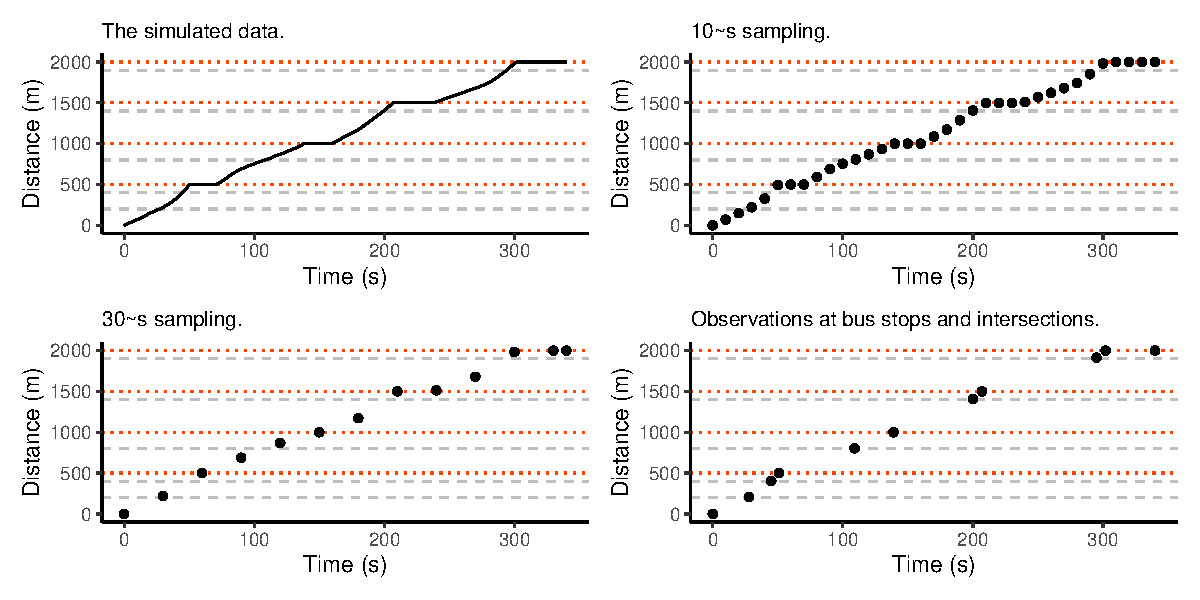
\includegraphics[width=.49\linewidth]{figure/sim2_graph-1} }
\subfloat[10~s sampling.\label{fig:sim2_graph2}]{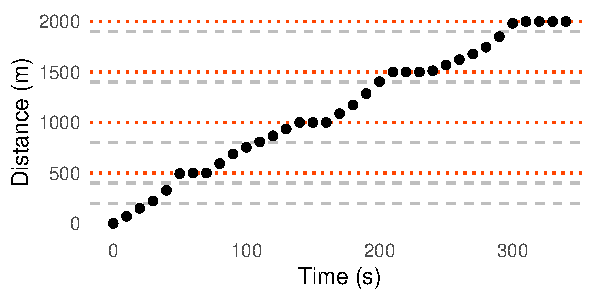
\includegraphics[width=.49\linewidth]{figure/sim2_graph-2} }\newline
\subfloat[30~s sampling.\label{fig:sim2_graph3}]{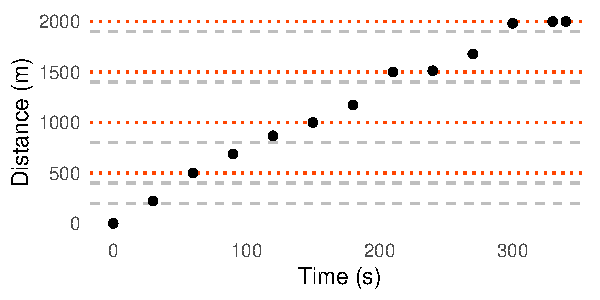
\includegraphics[width=.49\linewidth]{figure/sim2_graph-3} }
\subfloat[Observations at bus stops and intersections.\label{fig:sim2_graph4}]{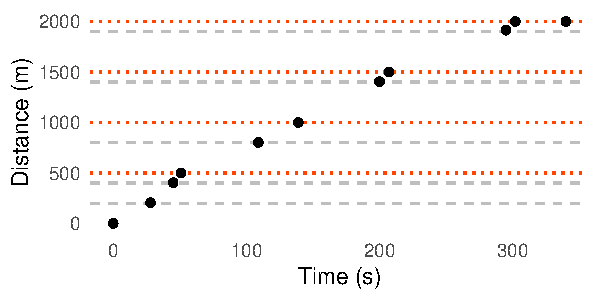
\includegraphics[width=.49\linewidth]{figure/sim2_graph-4} }\caption[Simulated vehicle trajectory, with five road segments and three intermediate stops]{Simulated vehicle trajectory, with five road segments and three intermediate stops.}\label{fig:sim2_graph}
\end{figure}


\end{knitrout}


The results of the second simulation are shown in \cref{fig:sim2_pf}, where we see somewhat similar results as before: the models perform similarly well under high-frequency uniform sampling, with lower precision under low-frequency sampling. For sampling at nodes, the models perform similarly.

\begin{knitrout}\small
\definecolor{shadecolor}{rgb}{0.969, 0.969, 0.969}\color{fgcolor}\begin{figure}
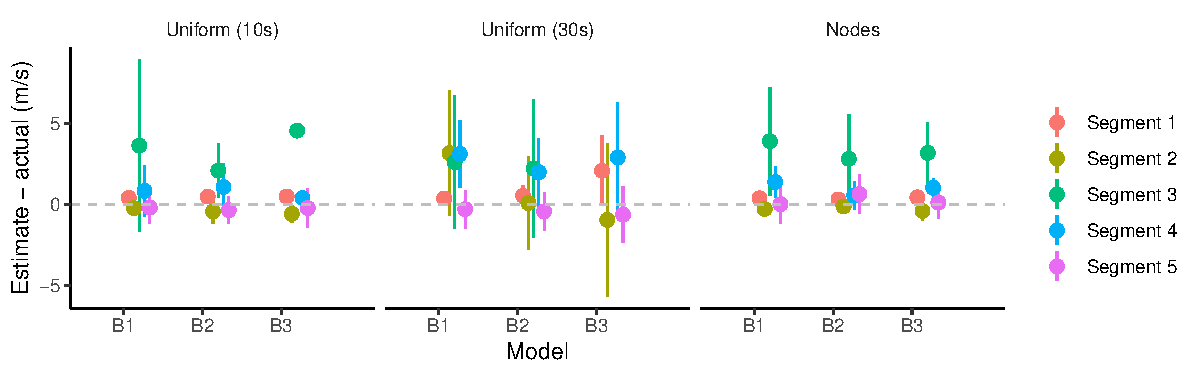
\includegraphics[width=\linewidth]{figure/sim2_pf-1} \caption[Simulation results for the three models (rows) applied to the data from three sampling methods (columns), using $\Np=2000$ particles]{Simulation results for the three models (rows) applied to the data from three sampling methods (columns), using $\Np=2000$ particles. [details].}\label{fig:sim2_pf}
\end{figure}


\end{knitrout}


Repeating the simulation 100~times with different vehicle trajectories, we can better compare the models (\cref{fig:sim2_pf_full}). Uncertainties are now much higher, on average, particularly under low-frequency sampling. The models all perform similarly, though A3 has the worst accuracy overall. \Cref{tab:sim2_pf_full} compares the estimates numerically using \gls{rmse} and \gls{mae}, where we see that within each sampling method the errors are similar. Models A1 and A2 perform similarly, while A3 is again consistently worse except under high-frequency sampling.


\begin{knitrout}\small
\definecolor{shadecolor}{rgb}{0.969, 0.969, 0.969}\color{fgcolor}\begin{figure}
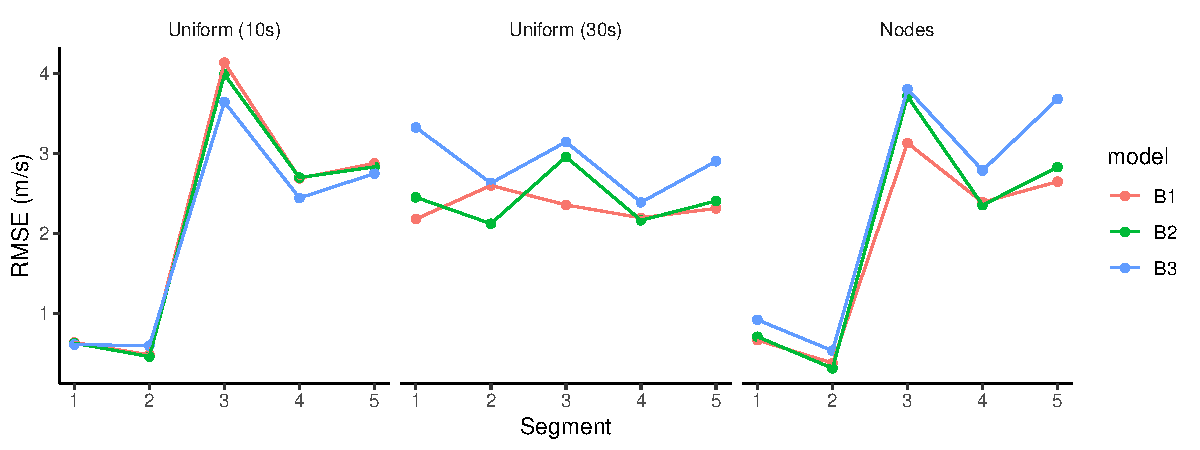
\includegraphics[width=\maxwidth]{figure/sim2_pf_full-1} \caption[Speed estimation results for 100 simulations]{Speed estimation results for 100 simulations. In each the vehicle trajectory is simulated using a different seed, and the speed estimate is taken as the mean of the particle speeds along each segment.}\label{fig:sim2_pf_full}
\end{figure}

\begin{table}

\caption{\label{tab:sim2_pf_full}RMSE of average speed estimation}
\centering
\fontsize{8}{10}\selectfont
\begin{tabular}[t]{llrr}
\toprule
Sampling method & Model & RMSE (m/s) & MAE (m/s)\\
\midrule
Uniform (10s) & A1 & 2.56 & 1.40\\
 & A2 & 2.51 & 1.35\\
 & A3 & 2.34 & 1.35\\
\midrule
Uniform (30s) & A1 & 2.34 & 1.58\\
 & A2 & 2.43 & 1.63\\
 & A3 & 2.90 & 2.14\\
\midrule
Nodes & A1 & 2.15 & 1.31\\
 & A2 & 2.36 & 1.35\\
 & A3 & 2.70 & 1.57\\
\bottomrule
\end{tabular}
\end{table}


\end{knitrout}






% \subsubsection{Simulation C: bus stops as nodes with unknown intersections}
% \label{sec:vehicle_sim_C}

% This time, we perform a simulation that more closely replicates the Auckland Transport system we are modelling. In it, we no longer know the locations of intersections, so road segments are specified between stops instead. In this simulation, the bus may still stop at intersections, but the underlying model does not know where these are. The goal is to esimate travel time along segments (which is now the \emph{link time} between stops).


% <<sim3_gen,echo=FALSE,message=FALSE>>=
% source("scripts/pf_simulation.R")
% sim3 <- run_simulation(
%     include = "both",
%     pr_stop = 0.5,
%     pr_int = 0,
%     noise = c(2.0, 5.0, 1),
%     prefix = "simC_results"
% )
% s3 <- sim3$sim

% segs <- lapply(1:nrow(s3$segments),
%     function(i) s3$segments$distance[i] + c(0, s3$segments$length[i])
% )
% tt <- s3$segments$tt

% fcap3 <- 'Simulated vehicle trajectory, with road segments as links between stops and unknown intersection locations'
% fscap3 <- c(
%     "The simulated data.",
%     "10~s sampling.",
%     "30~s sampling.",
%     "Observations at bus stops and intersections."
% )
% @

% \Cref{fig:sim3_graph} displays the simulated data in which only the stop locations are known, but the bus gets delays at intersections along the way. The results for this simulation are displayed in \cref{fig:sim3_pf}, which conveys that the \emph{uncertainty} is not being measured accurately (the speed tends to be underestimated).

% <<sim3_graph,echo=FALSE,fig.height=2,fig.width=4,out.width=".49\\linewidth",fig.cap=fcap2,fig.subcap=fscap2,fig.ncol=2,warning=FALSE,message=FALSE>>=
% p3 <- ggplot(s3$path, aes(time, distance)) +
%     geom_hline(yintercept = s3$segments$distance[-1],
%         lty = 2, colour = "gray") +
%     geom_hline(yintercept = s3$stops$distance[-1],
%         lty = 3, colour = "orangered") +
%     theme_minimal() +
%     theme(panel.grid = element_blank()) +
%     xlab('Time (s)') + ylab('Distance (m)') +
%     ylim(0, max(s3$path$distance)) + xlim(0, max(s3$path$time))

% p3 + geom_path()
% p3 + geom_point(aes(t, x), data = s3$observations$high)
% p3 + geom_point(aes(t, x), data = s3$observations$low)
% p3 + geom_point(aes(t, x), data = s3$observations$waypoints)
% @



% <<sim3_pf,echo=FALSE,message=FALSE,warning=FALSE,fig.height=3,fig.width=8,out.width="\\linewidth",fig.cap="Simulation results for the three models (rows) applied to the data from three sampling methods (columns), using $\\Np=2000$ particles. [details].">>=
% S0 <- sim3$fits
% S0 %>%
%     #% filter(segment != "Segment 4") %>%
%     mutate(
%         xpos = as.numeric(as.factor(model)) +
%             as.numeric(as.factor(segment)) / 15,
%         obs = factor(obs, labels = c("Uniform (10s)", "Uniform (30s)", "Nodes"))
%     ) %>%
%     ggplot(aes(xpos, speed_estimate - avg_speed, colour = segment)) +
%     geom_pointrange(
%         aes(
%             ymin = speed_estimate - avg_speed - speed_sd,
%             ymax = speed_estimate - avg_speed + speed_sd
%         ),
%         shape = 19, size = 0.5
%     ) +
%     facet_grid( ~ obs,  scales = "free_y") +
%     theme_classic() +
%     theme(strip.background = element_blank()) +
%     geom_hline(yintercept = 0, col = "gray", lty = 2) +
%     ylab("Estimate - actual (m/s)") +
%     scale_x_continuous(
%         "Model",
%         limits = c(0.5, 4.0),
%         breaks = 1:3,
%         labels = paste0("A", 1:3)
%     ) +
%     labs(colour = "")

% @



% <<sim3_pf_full,echo=FALSE,message=FALSE,warning=FALSE,fig.width=8,fig.height=5,fig.cap="Speed estimation results for 100 simulations. In each the vehicle trajectory is simulated using a different seed, and the speed estimate is taken as the mean of the particle speeds along each segment.">>=
% library(parallel)
% cl <- makeCluster(4L)
% r <- clusterEvalQ(cl, source("scripts/pf_simulation.R"))

% s00 <- pbapply::pblapply(1:100,
%     function(seed) {
%         run_simulation(seed = seed, include = "both", pr_stop = 0.5,
%             pr_int = 0.0,
%             prefix = "simC_results")
%     },
%     cl = cl
% ) %>%
%     map("fits") %>%
%     bind_rows() %>%
%     mutate(
%         model = factor(paste0("A", model)),
%         obs = factor(obs, labels = c("Uniform (10s)", "Uniform (30s)", "Nodes"))
%     )

% stopCluster(cl)

% s00 <- s00 %>%
%     filter(
%         # segment != "Segment 4" &
%         is.finite(speed_estimate) &
%         speed_estimate < 30
%     )

% p_base <- s00 %>%
%     group_by(obs, model, segment) %>%
%     summarize(
%         rmse = sqrt(
%             mean(
%                 (speed_estimate - avg_speed)^2,
%                 na.rm = TRUE
%             )
%         ),
%         mae = mean(
%             abs(speed_estimate - avg_speed),
%             na.rm = TRUE
%         )
%     ) %>%
%     mutate(
%         segment = as.integer(as.factor(segment))
%     ) %>%
%     ggplot(aes(x = segment, colour = model)) +
%         facet_grid(~obs) +
%         theme_classic() +
%         theme(strip.background = element_blank()) +
%         xlab("Segment")

% library(patchwork)
% prmse <- p_base +
%     geom_point(aes(y = rmse)) +
%     geom_path(aes(y = rmse)) +
%     ylab("RMSE (m/s)")
% pmae <- p_base +
%     geom_point(aes(y = mae)) +
%     geom_path(aes(y = mae)) +
%     ylab("MAE (m/s)")

% prmse / pmae

% s00 %>%
%     group_by(obs, model) %>%
%     summarize(
%         "RMSE (m/s)" = sqrt(
%             mean(
%                 (speed_estimate - avg_speed)^2,
%                 na.rm = TRUE
%             )
%         ) %>%
%             round(2),
%         "MAE (m/s)" = round(
%             mean(
%                 abs(speed_estimate - avg_speed),
%                 na.rm = TRUE
%             ),
%             2
%         )
%     ) %>%
%     ungroup() %>%
%     mutate(
%         rank = rank(obs, ties = "min"),
%         obs = as.character(obs),
%         obs = ifelse(seq_along(obs) == rank, obs, "")
%     ) %>%
%     select(-rank) %>%
%     rename(
%         "Sampling method" = obs,
%         "Model" = model
%     ) %>%
%     kable(
%         format = "latex",
%         booktabs = TRUE,
%         caption = "RMSE of average speed estimation",
%         escape = FALSE,
%         linesep = ""
%     ) %>%
%     kableExtra::row_spec(3, extra_latex_after = "\\midrule") %>%
%     kableExtra::row_spec(6, extra_latex_after = "\\midrule") %>%
%     kableExtra::kable_styling(font_size = 8)

% @



\phantom{\gls{rmse} \gls{mae}}
